Operations that are presented in $D$ can directly affect the complexity of consistency enforcement mechanisms. For example, if all operations are idempotent,  exactly-once can be achieved~\cite{Akidau:2013:MFS:2536222.2536229}. Among common types of operations, non-commutative ones provide significant difficulties in achieving exactly-once.

\begin{definition}{D contains non-commutative operation}
if\\ 
$\exists (x,y), s_1, s_2 \in \Gamma, s_1 \neq s_2: \\ ((x,y),s_1)\in D, \\ ((y,x),s_1)\notin D, \\ ((y,x),s_2)\in D$.
\end{definition}

The are many non-commutative operations that are commonly used in practice: concatenation, matrix multiplication, cross product, etc. Hence, general-purpose stream processing systems should support them. The problem with such operations we demonstrated above: simple reprocessing of missing elements in case of failure may lead to results inconsistencies.

\begin{definition}{System is deterministic}
if\\ 
$\forall{\tau\in{\mathbb{N}}, b_{\tau+1}\in{2^{\Gamma}}}:P(b_{\tau+1}|A_{\tau},B_\tau,F^{*})=1$.
\end{definition}

An essential property of a deterministic system is that it preserves the same order of elements before non-commutative operations on each run. We further demonstrate how this property can be used to achieve exactly-once with low performance overhead.

On the other hand, the absence of determinism imposes restrictions on exactly-once implementations. The following theorem denotes the necessary and sufficient conditions for exactly-once in non-deterministic systems with a non-commutative operation in $D$. It demonstrates that if a system is non-deterministic, but supports non-commutative operations, it must save (take a snapshot of) results of non-commutative operations before delivery of output elements that depend on these results.

\begin{figure}[t]
  \centering
  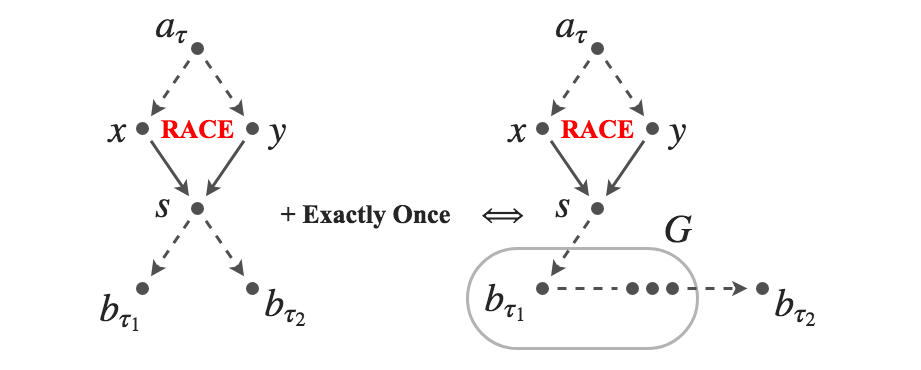
\includegraphics[width=0.8\textwidth]{Chapters/DeliveryGuarantees/pics/theorem-pic.png}
  \caption{The scheme of Theorem~\ref{necessary_conditions}}
  \label {theorem-pic}
\end{figure}

\begin{theorem}
\label{necessary_conditions}
If $D$ contains non-commutative transformation and has the following dependencies for some $a_\tau \in \Gamma$:

\begin{enumerate}
  \item[(i)] $x \in Cl_D(a_\tau), y \in Cl_D(a_\tau)$
  \item[(ii)] $((x,y),s)\in D$ through a non-commutative operation
  \item[(iii)] $b_{\tau_1}, b_{\tau_2} \in Cl_D(s), \tau_1 < \tau_2$
\end{enumerate}

\noindent then non-deterministic system supports exactly-once if and only if:

\begin{equation}
\label{theorem_conditions}
  \begin{gathered}
    G = Cl_D(b_{\tau_1}) \cap C_D^{-1}(b_{\tau_2}) \\
    \forall (u, v) \in D, u \in Cl_D(s): v \subset G \Rightarrow u \subset G
  \end{gathered}
\end{equation}

\end{theorem}
\begin{sketch}
$ $\newline

The scheme of the theorem is shown in Figure~\ref{theorem-pic}. The theorem conditions mean that each result of the non-commutative operation must become recoverable before the delivery of output that depends on this result. 
% Such behavior is similar to the issue shown in Ta~\ref{state-inconsistency} if we set $b_{\tau_1}=v$.
$ $\newline

\noindent{\em Necessary condition}\newline

  Assume that conditions~\ref{theorem_conditions} are not satisfied, i.e. $\exists v \subset G, u \not\subset G: (u, v) \in D$, and system fails at time $\tau_1<\tau_f<\tau_2$. Then, to obtain $b_{\tau_2}$ there is a need to recompute $v$, $u$ and therefore $s$. However, due to asynchronous distributed processing and non-commutative transformation, system can reach not exactly $s$ such that $((x,y), s) \in D$, but $s':((y,x),s')\in D$. In this case, after recovery element $b_{\tau_2}$ will be delivered, but it will depend not on $s$, but on $s'$: $b_{\tau_2}\in Cl_D(s')$. This is a contradiction, because $b_\tau$ has been already delivered and $P(b_{\tau_2}\in Cl_D(s')|\{a_\tau\},\{b_{\tau_1} \in Cl_D(s) \})=0$.
$ $\newline

\noindent{\em Sufficient condition}
\newline

Let us assume that a  system fails at time $\tau_f$. If $\tau_f < \tau_1$ or $\tau_f > \tau_2$,  exactly-once is obviously satisfied. Assume that $\tau_1<\tau_f<\tau_2$. In this case, $b_{\tau_1}\in B_{\tau_f}\subset B_{\tau_2}$. Hence, $b_{\tau_2}$ can be restored directly from $b_{\tau_1}$ without reprocessing of s, i.e. $F(a_\tau,b_{\tau_1})=b_{\tau_2}$ and $b_{\tau_1}, b_{\tau_2} \in Cl_D(s)$ after recovery, thus $P(b_{\tau_2}\in Cl_D(s)|\{a_\tau\},\{b_{\tau_1} \in Cl_D(s) \})>0$.
\end{sketch}


We assume   in this  theorem    that input element $a_\tau$ is split into elements $x,y$. The same behavior can be reproduced if two input elements $a_\tau$ and $a_{\tau+1}$ enter a system through asynchronous channels. In general, this behavior is natural for stream processing systems because elements are processed one-by-one without synchronization and order enforcement. 

This theorem has direct practical implications for non-deterministic systems:
\begin{itemize}
    \item {\bf Output elements must wait until the snapshot is taken}. If a system aims at providing exactly-once, it must output elements only if there exists a snapshot that contains results of non-commutative operations. The problem here is that a system is usually not aware of user-defined operations and cannot distinguish commutative and non-commutative operations, so it must wait even if all elements commutate.
    \item {\bf Latency is affected by the period of snapshotting}. The consideration above implies that the lower bound of latency in the worst case in non-deterministic systems is the snapshotting period, together with the duration of taking a snapshot. There is a trade-off between latency and the frequency of taking snapshots because too frequent snapshotting can cause high extra load, while rare snapshots lead to high latency.
\end{itemize}
